\documentclass[12pt,twoside]{toptesi}
\usepackage{listings}
\lstset{language=Java,breaklines=true,basicstyle=\footnotesize,frameround=fttt,frame=trBL}
\facolta[III]{Ingegneria}
\NomeMonografia{Relazione di progetto} 
\monografia{Automazione Discreta}
\corsodilaurea{Ingegneria Informatica}
\candidato{Luca \textsc{Belluccini}\\
	Piergiuseppe \textsc{Bettassa}\\
	Manuele \textsc{Bommarito}\\
	Matteo \textsc{Casalino}\\
	Davide \textsc{Ferri}\\
	Ivan \textsc{Lazzero}}
\sedutadilaurea{\textsc{Anno~accademico} 2008-2009}
\logosede{logopolito}
\includeonly{% 
	introduzione,%
	meccanica,%
	capitolo1, %
	%capitolo2,% 
	%capitolo3,% 
	%capitolo4% 
} 
\begin{document}\errorcontextlines=9
	\frontespizio
\indici
\sommario
Questo � il sommario
	\chapter{Meccanica del Robot}
Il robot � costituito da tre diverse parti funzionali: una base dotata di ruote motrici,
 un braccio rotante ed un sistema di leve a forbice.

\section{La base}
La base del robot � stata costruita partendo da un modello presente sul sito
della \emph{Lego}\textregistered 
(\emph{http://www.active-robots.com/products/mindstorms4schools/building-instructions/Build-RoboArm.pdf} Figura \ref{Base}) 
e modificato come segue: il motore B, che nello schema originale si occupava di far ruotare il braccio, continua nella sua funzione mentre il motore A
trasferisce la sua funzione da far muovere in avanti il braccio a gestire la trazione del robot.\\

\begin{figure}
	\begin{center}
		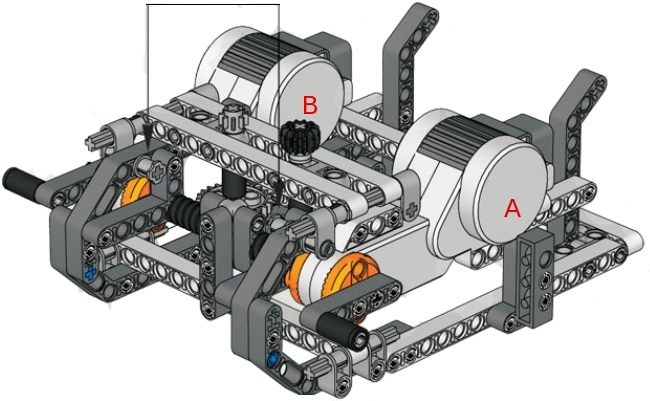
\includegraphics[scale=0.5]{img/base.png}
		\caption{Struttura iniziale della Base \label{Base}}
	\end{center}
\end{figure}

Per permettere al robot di avanzare, la base � stata montata su quattro ruote di
cui le due anteriori sono le ruote motrici. Quest'ultime sono collegate tra di
loro con un asse motore comune, che riceve il movimento tramite un gioco di
ingranaggi conici trasformando la rotazione dall'asse veticale, prodotta dal
motore A pi� la vite archimedea, in un movimento sull'asse orizzontale
necessario per l'avanzamento del robot.\\

Questo sistema ha per� mostrato delle carenze di precisione dovute da torsioni,
flessioni e giochi meccanici.\\

Per ovviare a ci� si � proceduto in pi� modi: 
\begin{itemize} 
  \item Creando un nuovo sistema di aggancio dell'albero motore verticale, in
 		 modo da minimizzarne la flessione. Nello specifico, si � inserita una
  		 piastrina triangolare per 'agganciare' l'albero motore, il pi� vicino
  		 possibile al punto di contatto tra gli ingranaggi conici. Figura
  		 \ref{ALBERO} FOTO ALBERO MOTORE 
  		 \begin{figure}
           \begin{center}
			 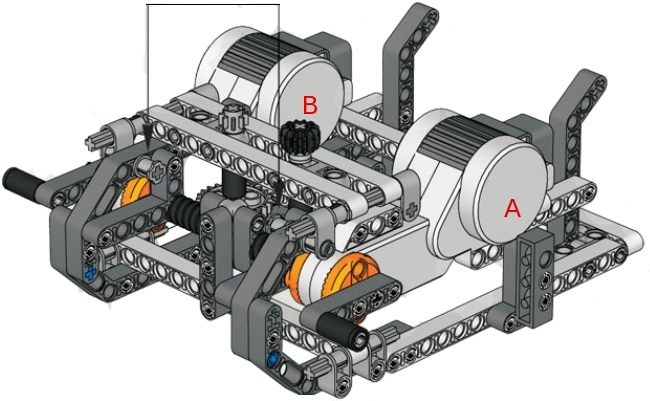
\includegraphics[scale=0.5]{img/base.png}
			 \caption{Struttura iniziale della Base \label{ALBERO}}
		   \end{center}		
		 \end{figure}
 
  \item Inserendo sotto la base un asse rigido che arrivi da ruota a ruota, in
  		 modo da ridurre la flessione dell'albero motore, dovuta al peso del robot
  		 stesso. \ref{SOSPENSIONI} FOTO SOSPENSIONI
 
		\begin{figure}
         \begin{center}
			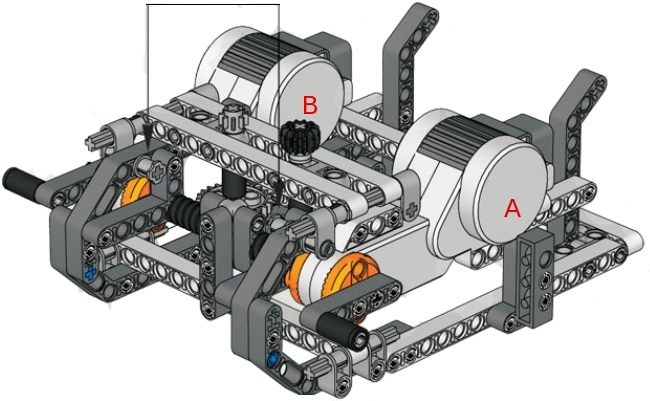
\includegraphics[scale=0.5]{img/base.png}
			\caption{Struttura iniziale della Base \label{SOSPENSIONI}}
		  \end{center}
		\end{figure} 

  \item Inserendo delle parti non non originali della 
  		\emph{Lego}\textregistered~per cercare di ridurre i giochi meccanici,
  		nello specifico si sono inserite delle rosette nella sede delle viti
  		achimedee e nei vari supporti degli assi. \ref{ROSETTE} FOTO ROSETTE
  		
  		\begin{figure}	
           \begin{center}	
			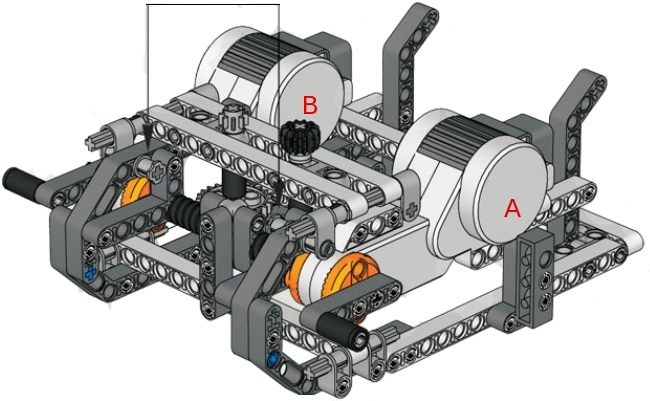
\includegraphics[scale=0.5]{img/base.png}
			\caption{Struttura iniziale della Base \label{ROSETTE}}
		  \end{center}			
		\end{figure}  	 


\end{itemize} 

Per i problemi relativi alle torsioni degli alberi non si � potuto fare nulla,
essendo questi problemi puramente dipendenti dalla natura fisica degli stessi e
non dal sistema di montaggio.

\section{Il Braccio}
Per la costrizione del braccio si � nuovamente presa ispirazione dalle
istruzioni della \emph{Lego}\textregistered~, modificandolo in modo da renderlo
rigido e non pi� snodabile Figura \ref{braccio} . Per effettuare questa
modifica si � elimitato il movimento centrale e fissati i montanti del braccio
tramite due 'traverse'.

  		\begin{figure}
          \begin{center}		
			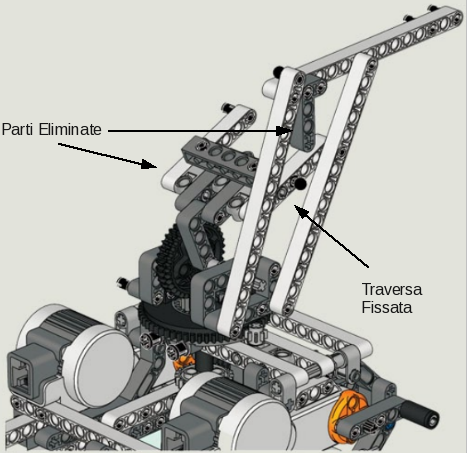
\includegraphics[scale=0.5]{img/braccio.png}
			\caption{Struttura del Braccio \label{braccio}}
		  \end{center}
		\end{figure} 

\section{Sistema di leve a forbice}
	\chapter{Il package Navigation}
Il \emph{package} \texttt{it.polito.Navigation} contiene le classi deputate a gestire i movimenti del Robot sulla scacchiera.\\
In particolare sono stati progettati due controllori: \texttt{CheckersNavigator} e\\ \texttt{ArmController} che sono responsabili rispettivamente della navigazione nelle due direzioni orizzontali e in quella verticale.\\
Di seguito si entrer� nel dettaglio delle implementazioni delle classi sopra
citate e dei relativi helper.
\section{La classe LashMotor}
I motori del NXT dispongono di un tachimetro incorporato, pertanto le API di
\emph{Lejos} mettono a disposizione una classe \texttt{Motor} che consente di
controllarli con una buona precisione. In particolare, mediante i metodi
\texttt{rotate()} e \texttt{rotateTo()}, � possibile ruotare il rotore di un
angolo arbitrario con un'incertezza di pi� o meno 2 gradi.\\
Per come sono stati impiegati i motori, tuttavia, si sono determinati dei giochi
meccanici non trascurabili tra il movimento dei rotori e lo spostamento effettivo
del Robot sulla scacchiera, che avrebbero causato errori di
posizionamento superiori alla lunghezza di mezza casella.\\
La classe \texttt{LashMotor} estende l'API \texttt{Motor} di \emph{Lejos} e
rappresenta un motore in grado di recuperare un gioco costante (che deve quindi
essere preventivamente stimato\footnote{La stima dei giochi � stata effettuata
empiricamente cercando di determinare l'angolo minimo tale da indurre un
movimento del Robot, in seguito a un cambio di verso di rotazione.}) in modo
trasparente all'utilizzatore.\\
Il metodo reimplementato in \texttt{LashMotor} � \texttt{rotateTo()}: il recupero
del gioco avviene solo quando si verifica un'inversione (si � scelto il verso
negativo perch� si richiede che i motori vengano inizializzati con gioco nullo
nel verso positivo, ad esempio a fine calibrazione) semplicemente
decrementando l'angolo di destinazione della costante \texttt{lash} stimata.\\
\begin{lstlisting}
	public void rotateTo(int limitAngle, boolean nonBlocking) {
		if (limitAngle < super.getTachoCount())
			limitAngle -= lash;
		super.rotateTo(limitAngle, nonBlocking);
	}
\end{lstlisting}
Si noti che, nel caso di cambio di direzione inverso, il recupero avviene senza
bisogno di modificare l'angolo di destinazione infatti, detti $c$ la costante
\texttt{lash} e $\theta_0$ l'angolo di partenza si avrebbe:
\begin{figure}[htbp]
	\begin{center}
		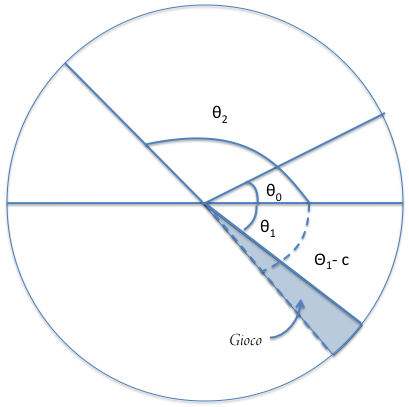
\includegraphics[scale=0.7]{img/lashMotor.png}
		\caption{Recupero dei giochi in un motore LashMotor \label{lashMotor}}
	\end{center}
\end{figure} 
\itemize
\item Rotazione all'angolo $\theta_1 < \theta_0$
	$$\theta = \theta_0 + (\theta_1 - \theta_0 - c) = \theta_1 - c$$
\item Rotazione all'angolo $\theta_2 > \theta_1$
	$$\theta = \theta_1 - c + (\theta_2 - (\theta_1 - c)) = \theta_2$$

\section{L'interfaccia  CheckersNavigator}
Questa interfaccia astrae le funzionalit� di movimento bidimensionale sulla scacchiera 8x8; i metodi pi� importanti sono:

\begin{lstlisting}
/** Ritorna la posizione X [0; 7] */
public int getX(); 
/** Ritorna la posizione Y [0; 7] */
public int getY(); 
/** Muove il braccio sulla casella (X, Y) */
public void goTo(int newX, int newY) throws NotCalibratedException; 
/** Muove il braccio sulla casella "base" */
public void goHome() throws NotCalibratedException; 
/** Modifica la velocit� dei motori */
public void setSpeed(int speedA, int speedB);
/** Effettua la calibrazione */
public void calibrate();
\end{lstlisting}
Si noti come i metodi che comportano un movimento non possano essere eseguiti se prima non � stata effettuata la calibrazione (eccezione \texttt{NotCalibrated\-Exception}).\\
Esamineremo ora le implementazioni che sono state progettate per questa interfaccia.

\subsection{La classe SimpleNavigator}
Questa prima implementazione si basa su un mapping statico di tutte le caselle relativo ad un punto iniziale su cui il Robot tenta di posizionarsi in fase di calibrazione.

\paragraph{Calibrazione}
Il Robot, per come � costruito, pu� ruotare il suo braccio agendo sul motore B, o
pu� spostarlo avanti e indietro agendo sul motore A.\\ Il primo metodo di
calibrazione che � stato pensato, � pertanto semplicemente mirato a portare il
braccio in una posizione nota (punto rosso in Figura \ref{simpleNavigatorGrid}),
in modo da poter usare offset predeterminati (relativi ad essa) per spostarlo su
tutte le altre caselle. \\ \begin{figure}[ht]
\begin{center}
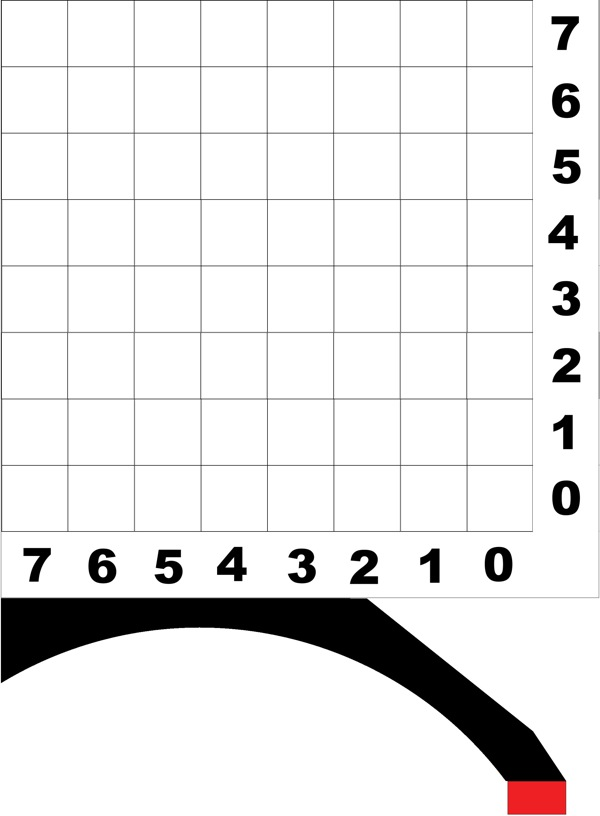
\includegraphics{img/simpleNavigatorGrid.jpg}
\caption{Scacchiera SimpleNavigator \label{simpleNavigatorGrid}}
\end{center}
\end{figure}
Il metodo \texttt{calibrate()} non fa altro che ruotare il braccio verso destra finch� il sensore di colore montato su di esso non rileva il colore rosso, a quel punto recupera eventuali giochi dei motori e azzera i contatori di distanza angolare in essi contenuti.

\paragraph{Navigazione}
Gli angoli di destinazione cui vengono fatti ruotare i motori sono calcolati semplicemente come\footnote{X e Y sono rispettivamente le  coordinate di ascissa e di ordinata delle caselle}: 
\begin{lstlisting}
destAngleA = offA+posy[newY]+dely[newX];
destAngleB = offB+posx[newX];
\end{lstlisting}
I vettori \texttt{posx} e \texttt{posy} definiscono l'offset in funzione delle rispettive coordinate;
il vettore \texttt{dely} contiene le correzioni da effettuare sull'asse y in funzione della coordinata x,
in modo da recuperare gli scostamenti in verticale dati dal fatto che il braccio si muove su un arco
di circonferenza.\\
Le costanti \texttt{offA} e \texttt{offB} definiscono invece l'offset necessario a portare il braccio
sulla casella (5,0) che costituiva il punto pi� comodo cui riferire la taratura di tutte le altre caselle.

\subsection{La classe MathNavigator}
Il limite pi� evidente del \texttt{SimpleNavigator} � dato dai vincoli statici di allineamento
che devono sussistere tra Robot e scacchiera. \'E chiaro infatti che, nel caso in cui non si
posizionasse il braccio in modo da far coincidere il suo centro di rotazione con il centro del
tratto di circonferenza in Figura \ref{simpleNavigatorGrid}, questo non riuscirebbe a seguire l'arco stesso
in fase di calibrazione e non potrebbe quindi successivamente posizionarsi sulla scacchiera.\\
Per ovviare a questo fatto � stato introdotto un modello geometrico del sistema, in modo da avere a
disposizione una soluzione analitica del problema.\\
Di nuovo andremo ad illustrare separatamente le fasi di calibrazione e di navigazione che, in questo caso,
risultano ovviamente pi� complesse.
\paragraph{Calibrazione}
La costruzione cui si far� riferimento nel seguito � quella in Figura \ref{mathNavigator1}, in cui si possono
osservare la scacchiera quadrata di lato $l$ e la circonferenza di centro $C$ e raggio $r$ descritta dal braccio
che si muove su di essa.\\
\begin{figure}[ht]
\begin{center}
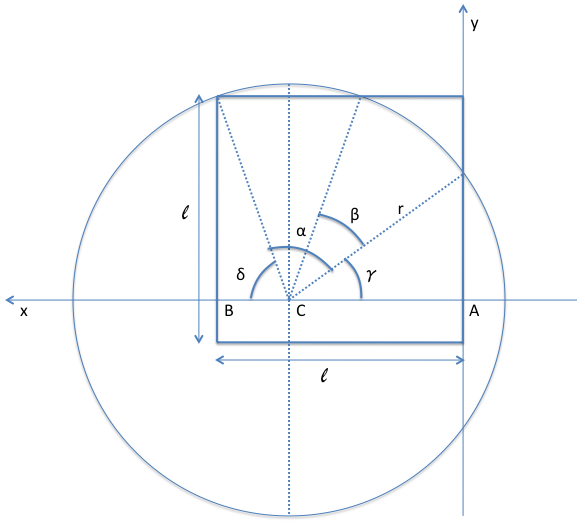
\includegraphics[scale=0.65]{img/mathNavigator1.png}
\caption{Calibrazione MathNavigator \label{mathNavigator1}}
\end{center}
\end{figure}
L'idea � quella di permettere al Robot di determinare il rapporto $\frac{\overline{BC}}{\overline{CA}}$
(e quindi la posizione del suo centro rispetto alla scacchiera) a partire dalla misura, eseguita in fase di
calibrazione mediante i sensori disponibili, di parametri geometrici.\\
Il parametro pi� comodo da misurare, semplicemente usando il sensore di colore e il tachimetro interno ai motori,
� quello che in Figura \ref{mathNavigator1} � indicato come angolo $\alpha$, cio� l'angolo descritto dal braccio
quando sorvola l'intera scacchiera. Una volta determinato $\alpha$ e
ipotizzando $\overline{BC}<\overline{CA}$ si pu� risolvere il problema in forma chiusa:
$$\delta = \frac{\pi - \alpha + \beta}{2}$$
$$\gamma = \delta - \beta$$
$$l = r(\cos\gamma+\cos\delta) = r(\cos(\frac{\pi-\alpha+\beta}{2})+\cos(\frac{\pi-\alpha+\beta}{2}-\beta)) =$$
$$= r ( \cos(\frac{\pi-\alpha}{2})\cos(\frac{\beta}{2}) - \sin(\frac{\pi-\alpha}{2})\sin(\frac{\beta}{2}) +
\cos(\frac{\pi-\alpha}{2})\cos(\frac{\beta}{2}) + \sin(\frac{\pi-\alpha}{2})\sin(\frac{\beta}{2}) ) =$$
$$= 2r\cos(\frac{\pi-\alpha}{2})\cos\frac{\beta}{2}$$
$$\beta = 2\arccos(\frac{l}{2r\cos(\frac{\pi-\alpha}{2})})  = 2\arccos(\frac{l}{2r\sin\frac{\alpha}{2}})$$
$$\overline{CA} =  r\sin(\frac{\alpha+\beta}{2})$$ 
\paragraph{Navigazione}

\section{La classe ArmController}
 
	\include{capitolo2} 
	\include{capitolo3} 
	\include{capitolo4} 
\end{document}
